\documentclass[conference]{IEEEtran}

\usepackage[numbers, sort, compress]{natbib}
\usepackage{graphicx}
\usepackage{amsmath}
\usepackage{amssymb}
\usepackage{color}
\usepackage{ifpdf}

\usepackage{dcolumn}
\usepackage{float}
\usepackage[utf8]{inputenc}
\usepackage{multirow}
\usepackage{rotating}

\usepackage[tight]{subfigure}



%\usepackage[numbers, sort, compress]{natbib}
%\usepackage{latex8}
%\usepackage{float}
%\usepackage{times}    
\usepackage{url}
\usepackage{listings}   
\usepackage{paralist}    
\usepackage{wrapfig}    
%\usepackage[small,it]{caption}
\usepackage{multirow}
\usepackage{ifpdf}
%\usepackage{srcltx}
%\usepackage{subfigure}
\usepackage{xspace}
\usepackage{keyval}  
\usepackage{color}

\definecolor{listinggray}{gray}{0.95}
\definecolor{darkgray}{gray}{0.7}
\definecolor{commentgreen}{rgb}{0, 0.4, 0}
\definecolor{darkblue}{rgb}{0, 0, 0.4}
\definecolor{middleblue}{rgb}{0, 0, 0.7}
\definecolor{darkred}{rgb}{0.4, 0, 0}
\definecolor{brown}{rgb}{0.5, 0.5, 0}

\usepackage[normalem]{ulem}
\makeatletter
\def\cyanuwave{\bgroup \markoverwith{\lower3.5\p@\hbox{\sixly \textcolor{cyan}{\char58}}}\ULon}
\def\reduwave{\bgroup \markoverwith{\lower3.5\p@\hbox{\sixly \textcolor{red}{\char58}}}\ULon}
\def\blueuwave{\bgroup \markoverwith{\lower3.5\p@\hbox{\sixly \textcolor{blue}{\char58}}}\ULon}
\font\sixly=lasy6 % does not re-load if already loaded, so no memory problem.
\makeatother

%!TEX root = sc12/pstar-sc2012-ieee.tex
\newif\ifdraft
%\drafttrue
\ifdraft
\newcommand{\onote}[1]{ {\textcolor{cyan} { (***Ole: #1) }}}
\newcommand{\terminology}[1]{ {\textcolor{red} {(Terminology used: \textbf{#1}) }}}
\newcommand{\owave}[1]{ {\cyanuwave{#1}}}
\newcommand{\jwave}[1]{ {\reduwave{#1}}}
\newcommand{\alwave}[1]{ {\blueuwave{#1}}}
\newcommand{\jhanote}[1]{ {\textcolor{red} { ***shantenu: #1 }}}
\newcommand{\alnote}[1]{ {\textcolor{blue} { ***andreL: #1 }}}
\newcommand{\amnote}[1]{ {\textcolor{blue} { ***andreM: #1 }}}
\newcommand{\smnote}[1]{ {\textcolor{brown} { ***sharath: #1 }}}
\newcommand{\msnote}[1]{ {\textcolor{cyan} { ***mark: #1 }}}
\newcommand{\note}[1]{ {\textcolor{magenta} { ***Note: #1 }}}
\else
\newcommand{\onote}[1]{}
\newcommand{\terminology}[1]{}
\newcommand{\owave}[1]{#1}
\newcommand{\jwave}[1]{#1}
\newcommand{\alnote}[1]{}
\newcommand{\amnote}[1]{}
\newcommand{\athotanote}[1]{}
\newcommand{\smnote}[1]{}
\newcommand{\jhanote}[1]{}
\newcommand{\msnote}[1]{}
\newcommand{\note}[1]{}
\fi

\newcommand{\pilot}{Pilot\xspace}
\newcommand{\pilots}{Pilots\xspace}
\newcommand{\pilotjob}{Pilot-Job\xspace}
\newcommand{\pilotjobs}{Pilot-Jobs\xspace}
\newcommand{\computeunit}{Compute Unit\xspace}
\newcommand{\computeunits}{Compute Units\xspace}
\newcommand{\cu}{CU\xspace}
\newcommand{\cus}{CUs\xspace}
\newcommand{\cs}{Compute Service\xspace}
\newcommand{\css}{Compute Services\xspace}
\newcommand{\pcs}{Pilot Compute Service\xspace}
\newcommand{\dataunit}{Data Unit\xspace}
\newcommand{\dataunits}{Data Unit\xspace}
\newcommand{\du}{DU\xspace}
\newcommand{\dus}{DUs\xspace}
\newcommand{\pilotdata}{Pilot-Data\xspace}
\newcommand{\pd}{PD\xspace}
\newcommand{\pds}{Pilot Data Service\xspace}
\newcommand{\pdss}{Pilot Data Services\xspace}
\newcommand{\su}{SU\xspace}
\newcommand{\sus}{SUs\xspace}
\newcommand{\schedulableunit}{Schedulable Unit\xspace}
\newcommand{\schedulableunits}{Schedulable Units\xspace}
\newcommand{\cc}{c\&c\xspace}
\newcommand{\CC}{C\&C\xspace}

\lstdefinestyle{myListing}{
  frame=single,   
  backgroundcolor=\color{listinggray},  
  %float=t,
  language=C,       
  basicstyle=\ttfamily \footnotesize,
  breakautoindent=true,
  breaklines=true
  tabsize=2,
  captionpos=b,  
  aboveskip=0em,
  belowskip=-2em,
  %numbers=left, 
  %numberstyle=\tiny
}      

\lstdefinestyle{myPythonListing}{
  frame=single,   
  backgroundcolor=\color{listinggray},  
  %float=t,
  language=Python,       
  basicstyle=\ttfamily \footnotesize,
  breakautoindent=true,
  breaklines=true
  tabsize=2,
  captionpos=b,  
  %numbers=left, 
  %numberstyle=\tiny
}

\newcommand{\up}{\vspace*{-1em}}
\newcommand{\upp}{\vspace*{-0.5em}}
\newcommand{\numrep}{8 }
\newcommand{\samplenum}{4 }
\newcommand{\tmax}{$T_{max}$ }
\newcommand{\tc}{$T_{C}$ }
\newcommand{\tcnsp}{$T_{C}$}
\newcommand{\bj}{BigJob}

%  \setlength{\parskip}{0.05ex} % 1ex plus 0.5ex minus 0.2ex}
%  \setlength{\parsep}{0pt}
%  %\setlength{\headsep}{0pt}
%  \setlength{\topskip}{0pt}
%  \setlength{\topmargin}{0pt}
%  %\setlength{\topsep}{0pt}
%  \setlength{\partopsep}{0pt}

% This is now the recommended way for checking for PDFLaTeX:


\ifpdf
\DeclareGraphicsExtensions{.pdf, .jpg, .tif}
\else
\DeclareGraphicsExtensions{.eps, .jpg}
\fi

\tolerance=1000
\hyphenpenalty=10


\begin{document}
%
%
%
%
%
%

\title{P*: A Model of Pilot-Abstractions}

\author{
  Andre Luckow$^{1}$, Mark Santcroos$^{2,1}$, Ole Weidner$^{1}$, Andre Merzky$^{1}$, Pradeep Mantha$^{1}$, Shantenu Jha$^{3,1*}$\\[0.4em]
  \small{\emph{$^{1}$Center for Computation \& Technology, Louisiana State University, USA}}\\[-0em]
  \small{\emph{$^{2}$Bioinformatics Laboratory, Academic Medical Center, University of Amsterdam, The Netherlands}}\\[-0em]
  \small{\emph{$^{3}$ Rutgers University, Piscataway, NJ 08854, USA}}\\[-0em]
%
  \small{\emph{$^{*}$Contact Author: \texttt{shantenu.jha@rutgers.edu}}}\\[-0.3em]
  \up\up}

\date{}
\maketitle

\begin{abstract} 

 %
  %
  %
  %
  %
  %
  %

  \pilotjobs support effective distributed resource utilization, and
  are arguably one of the most widely-used distributed computing
  abstractions -- as measured by the number and types of applications
  that use them, as well as the number of production distributed
  cyberinfrastructures that support them.  In spite of broad uptake,
  there does not exist a well-defined, unifying conceptual model of
  \pilotjobs which can be used to define, compare and contrast
  different implementations.  Often \pilotjob implementations are
  strongly coupled to the distributed cyberinfrastructure they were
  originally designed for. 
  %
  %
  These factors present a barrier to extensibility and
  interoperability. This paper is an attempt to (i) provide a minimal
  but complete model (P*) of \pilotjobs, (ii) establish the generality
  of the P* Model by mapping various existing and well known \pilotjob
  frameworks such as Condor and DIANE to P*, (iii) derive an
  interoperable and extensible API for the P* Model (Pilot-API), (iv)
  validate the implementation of the Pilot-API by concurrently using
  multiple distinct \pilotjob frameworks on distinct production
  distributed cyberinfrastructures, and (v) apply the P* Model to
  \pilotdata.
\end{abstract}
%
%
%
%

%

\section{Introduction and Overview} 

%

The seamless uptake of distributed infrastructures by scientific applications
has been limited by the lack of pervasive and simple-to-use abstractions at
multiple levels -- at the development, deployment and execution
stages~\cite{dpagrid2009-short}. Even where meaningful abstractions exist, the
challenges of implementing them in an extensible, reliable and scalable
manner, so as to support multiple applications are formidable. The lack of
appropriate implementations has in fact resulted in ``one-off'' solutions that
address challenges in a highly customized manner. Tools and implementations
are often highly dependent on and tuned to a specific execution environment,
further impacting portability, reusability and extensibility. Semantic and
interface incompatibility are certainly barriers, but so is the lack of a
common architecture and conceptual framework upon which to develop similar
tools a barrier. This general state of affairs also captures the specific
state of the abstractions provided by {\it \pilotjobs (PJ)}. There are a
plethora of working definitions and roles for \pilotjobs; from our
perspective, a \pilotjob provides the ability to utilize a placeholder job as
a container for a dynamically determined set of compute tasks.

%
%
%
%

Distributed cyber/e-infrastructure is by definition comprised of a set
of resources that is fluctuating -- growing, shrinking, changing in
load and capability (in contrast to a static resource utilization
model of traditional parallel and cluster computing systems).  The
ability to utilize a dynamic resource pool is thus an important
attribute of any application that needs to utilize distributed
cyberinfrastructure (DCI) efficiently. As a consequence of providing a
simple approach for decoupling workload management and resource
assignment/scheduling, PJ provide an effective abstraction for dynamic
execution and resource utilization in a distributed context.  Not
surprisingly, \pilotjobs have been one of the most successful
abstractions in distributed computing.  The fundamental reason for the
success of the \pilotjob abstraction is that \pilotjobs liberate
applications/users from the challenging requirement of mapping
specific tasks onto explicit heterogeneous and dynamic resource pools.
\pilotjobs thus shield applications from having to load-balance tasks
across such resources.  The \pilotjob abstraction is also a promising
route to address specific requirements of distributed scientific
applications, such as coupled-execution and application-level
scheduling~\cite{ko-efficient-short,DBLP:conf/hpdc/KimHMAJ10}.


A variety of PJ frameworks have emerged: Condor-G/
Glide-in~\cite{condor-g}, Swift~\cite{Wilde2011},
DIANE~\cite{Moscicki:908910}, DIRAC~\cite{1742-6596-219-6-062049},
PanDA~\cite{1742-6596-219-6-062041}, ToPoS~\cite{topos},
Nimrod/G~\cite{10.1109/HPC.2000.846563}, Falkon~\cite{1362680} and
MyCluster~\cite{1652061}, to name a few. Although they are all, for
the most parts, functionally equivalent -- they support the decoupling
of workload submission from resource assignment -- it is often
impossible to use them interoperably, or even just to compare them
functionally or qualitatively.
%
%
%
%
%
%
%
%
%

%
%

%
%

%
%
%

%
%
%
%


%
%
%
%

%
%
%
%
%
%
%


%
%
%
%
%

%
%
%

%
%

Our objective is to provide a minimal, but complete model for \pilot
abstractions~\cite{pstar-2012} -- referred to as P* Model ("P-star"),
which we present in \S\ref{sec:pilot-model}. The P* Model provides a
conceptual basis to compare and contrast different PJ frameworks --
which to the best of our knowledge is the first such attempt.  We also
investigate generalizations to the base P* Model: a natural and
logical extension of the P* Model arises from the opportunity to
extend it to include data in addition to computational tasks. This
leads to an abstraction analogous to the \pilotjob: the
\emph{\pilotdata (PD)} abstraction. The potentially consistent
treatment of data and compute suggests symmetrical compute and data
elements in the model; thus we refer to this model as the P* Model of
Pilot Abstractions.

%
%
%

In \S\ref{sec:pilot-job-frameworks} we validate the P* Model by
analyzing well-known PJ frameworks (BigJob, Condor-G/Glide-in, DIANE)
and mapping them to the elements of the P* Model.
%
\S\ref{sec:pilot-api} of this paper motivates
and describes the Pilot-API; we discuss how existing and widely used
\pilotjob frameworks can be used through the
Pilot-API. \S\ref{sec:exp_res} describes the experiments and
performance measurements used to characterize the workings of the
Pilot-API and to demonstrate interoperability across middleware and
infrastructure. %
To further substantiate the impact of P*, we will demonstrate
interoperability between different PJ frameworks. %
We believe this is also the first demonstration of concurrent
interoperation of different \pilotjob implementations. Performance
advantages arising from the ability to distribute part of a
data-intensive workload are discussed; interoperable capabilities
increase flexibility in resource selection and optimization.

It is worth noting that \pilotjobs are used on every major national
and international DCI, including NSF/XSEDE, NSF/DOE Open Science Grid
(OSG), European Grid Initiative (EGI) and others; they are used to
support hundreds of thousands of tasks daily. Thus we believe the
impact and validation of this paper lies in its ability to not only
influence but also bridge the theory and practice of \pilotjobs, and
thus multiple domains of science dependent on distributed
cyberinfrastructure.


\section{The P* Model of Pilot-\\Abstractions}
\label{sec:pilot-model}

An initial motivation for the P* Model of pilot-abstractions is to
provide a common analytical framework to understand commonly
used \pilotjob frameworks.  The P* model was derived by analyzing many
\pilotjob implementations.  We first present
the common {\it elements} of the P* Model, followed by a description
of the {\it characteristics} that determine the interaction of these
elements and the overall functioning of any \pilotjob framework 
consistent with the P* Model.  

Before we proceed to discuss the P* Model, it is important to
emphasize that there exists a plethora of terms (abstraction,
model, framework, implementation etc) that are overloaded and
overlapping, and often used inconsistently in the literature;
thus we establish context and usage of relevant terms.

%
%

\B{\I{Terms and Usage:}} A \pilotjob can be defined as an \emph{
  abstraction} that generalizes the reoccurring concept of utilizing a
placeholder job as a container for a set of compute tasks; an instance
of that placeholder job is commonly referred to as \emph{\pilotjob}
or \emph{pilot}. The P* \emph{model} provides a %
comprehensive description of the \pilotjob abstraction, based on a set of
identified elements and their interactions. The P* Model can be used
as a {\it conceptual model}, for analyzing different implementations
of the \pilotjob abstraction. The \emph{Pilot-API} provides an
interface that exposes a sub-set of the P* elements and
characteristics to applications.  It is important to distinguish P* --
which provides a conceptual (abstract) model, from an implementation
of the P* Model. A \emph{\pilotjob framework} refers to a specific
instance of a \pilotjob implementation
that provides the complete \pilotjob functionality (e.\,g.\
BigJob).

%
%
%
%
%
%
%

%
%

\begin{figure}[t]
    \centering
    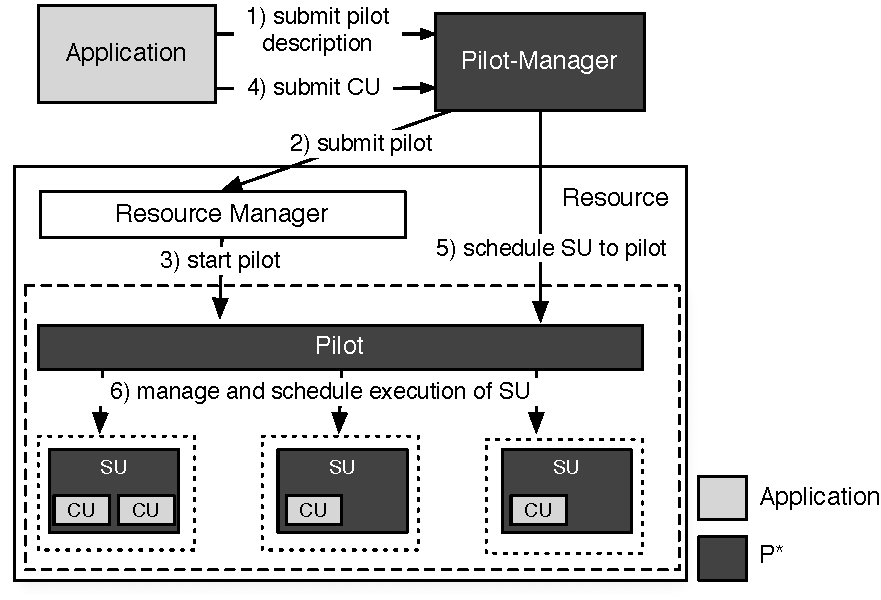
\includegraphics[width=0.48\textwidth]{figures/pstar_model_single.pdf}
    \caption{\I{\textbf{P* Model: Elements, Characteristics and
        Interactions:} The manager has two functions: it manages 1)
      Pilots (step 1-3) and 2) the execution of \cus. After a \cu is
      submitted to the manager, it transitions to an \su, which is
      scheduled to a \pilot by the PM. 
     %
   }\up\up}
    \label{fig:figures_pstar}
\end{figure}

%
%

  %
  %
  %
  %
  %

%
%
%

\noindent 
\subsection{Elements of the P* Model}

\noindent This sub-section defines the elements of the P* Model:

\noindent$\bullet$ \textbf{\pilot (Pilot-Compute):} The \pilot is the
entity that actually gets submitted and scheduled on a resource.  The
Pilot provides
application (user) level control and management of the set of
allocated resources.

%
%
%
%
%
%

\noindent$\bullet$ \textbf{\computeunit  (\cu):} A \cu  encapsulates a 
  self-contained piece of work (a compute task) specified by the application, that is
  submitted to the \pilotjob framework. There is no intrinsic notion
  of resource associated with a \cu.

\noindent$\bullet$ \textbf{Scheduling Unit (SU):} SUs are the units of 
  scheduling, internal to the P* Model, i.e., it is not known by or
  visible to an application. Once a \cu is
  under the control of the \pilotjob framework, it is assigned
  to an SU.
  %
  %
  %
%
%
%

\noindent$\bullet$ \textbf{Pilot-Manager (PM):} The PM is responsible for (i)
  orchestrating the interaction between the \pilots as well as the
  different components of the P* Model (\cus, \sus) and (ii) decisions
  related to internal resource assignment (once resources have been
  acquired by the \pilotjob).  For example, an SU can consist of one
  or more \cus. Further, \cus and \sus can be combined and aggregated;
  the PM determines how to group them, when \sus are scheduled and
  executed on a resource via the \pilot, as well as how many resources
  to assign to an SU.

  %
  %


%
%
%
%
%

%
%
%


%
%
%

  
  The application utilizes a PJ framework to execute multiple
  instances (ensemble) of an application kernel (kernel: 
  the actual binary that gets executed), or
  alternatively instances of multiple different application kernels (a
  workflow).  To execute an application kernel, an application must
  define a \cu specifying the application kernel as well as other
  parameters. This \cu is then submitted to the PM (the entry point to
  the \pilotjob framework), where it transitions to an \su. The PM is
  then responsible for scheduling the \su onto a \pilot and then onto
  a physical resource.  As we will see in
  \S\ref{sec:pilot-job-frameworks}, the above elements can be mapped
  to specific entities in many existing \pilotjob frameworks --
  more than one logical element are often rolled into
  one specific entity in a \pilotjob.

%
%
%
%
%
%
%
%
%
%
%
%
%
%
%
%


\subsection{Characteristics of P* Model}
\label{sec:p_star_elements}

%

%
%
%
%
%
%
%
%
%
 
We propose a set of fundamental properties/characteristics that
describe the interactions between the elements, and thus aid in the
description of P* Model.

%
%
%
%

\textbf{Coordination Characteristics:} these describe how
various elements of the P* Model, i.\,e.\ the PM, the \pilot, the \cus
and the SUs, interact. A common coordination pattern is master/worker
(M/W): the PM represents the master process that controls a set of
worker processes, the \pilots. The point of decision making is the
master process. In addition to the \emph{centralized} M/W, M/W can
also be deployed \emph{hierarchically}.  Alternatively, coordination
between the elements, in particular the \pilots, can be performed so as
to be \emph{decentralized}, i.\,e.\ without central decision making
point.

%

\textbf{Communication Characteristics:} The communication characteristics describes the
mechanisms for data exchange between the elements of the P* Model:
e.\,g.\ messages (point-to-point, all-to-all, one-to-all, all-to-one,
or group-to-group), streams (potentially unicast or multicast),
publish/subscribe messaging or shared data spaces.
		
\textbf{Scheduling Characteristics:} describe the process of mapping a \su to 
resources via a \pilot, and potential multiple levels of scheduling. Scheduling 
has a spatial component (which \su is executed on which \pilot?) but also a 
temporal component (when to bind?). For example, for the temporal component: a 
\su can be bound to a \pilot either before the \pilot has in turn been 
scheduled ({\it early} binding), or binding occurs if the \su is bound after 
the \pilot has been scheduled ({\it late} binding).
The different scheduling decisions that need to be made are representative of 
multi-level scheduling that is often required in distributed environments. For 
example, the \pilot is scheduled using the {\it system-level} scheduler. Once 
resources are assigned to the \pilot, {\it application-level} scheduling can 
occur at several levels both inside and outside the PJ framework.


%
%

The term {\it agent}, although not a part of the P* Model, finds
mention when discussing implementations. For the purposes of this
paper, an agent refers to a ``proxy process'' 
%
that has some decision making capability, and could aid the
implementation of one or more of the characteristics of the P* Model
(coordination, communication, scheduling), within a \pilotjob
framework.  These agents can be used to enforce a set of
(user-defined) policies (e.g.  resource capabilities, data/compute
affinities, etc.) and heuristics.




\subsection{P* as a Model for Pilot-Data}
\label{sec:pilot-data}
%
%

%
%

%
%
%


Many scientific applications have immense data requirements, which are
projected to increase dramatically in the near future~\cite{hey2009}. 
%
%
While \pilotjobs efficiently support late-binding of
\I{\computeunits} and resources, the analogous management of data in
distributed systems remains a challenge due to various reasons: (i) the
placement of data is often decoupled from the placement of Compute Units and
Pilots, i.\,e.\ the application must often manually stage in and out its data
using simple scripts; (ii) heterogeneity, e.\,g.\ with respect to storage,
filesystem types and paths, often prohibits or at least complicates late
binding decisions; (iii) higher-level abstraction that allow applications to
specify their data dependencies on an abstract, logical level (rather than on
file basis) are not available; (iv) due to lack of a common treatment for
compute and data, optimizations of data/compute placements are often not
possible.
%
%
%
%

%
%
%
%
%
%
%
%

%

This motivates an analogous abstraction that we call \emph{\pilotdata
  (PD)}. PD provides late-binding capabilities for data by
separating the allocation of physical storage and application-level
data units. Further, it provides an abstraction for expressing and
managing relationships between data units and/or compute units. These
relationships are referred to as \emph{affinities}.

%
%

%
\subsubsection*{P* Model Elements for Data}

%
%

The elements defined by P* can be extended with the following elements:

%

\noindent$\bullet$
  \textbf{\pilot (Pilot-Data):} A \pilotdata (\pd) functions as a 
	placeholder object that reserves the space
	for data units. PD facilitates the late-binding of data and resource and is
	equivalent to the \pilot in the compute model.

\noindent$\bullet$
  \textbf{Data Unit (DU):} DU is the base unit of data assigned by
  the application,  e.\,g.\ a set of data files. 
%

%
%
%
%

\noindent$\bullet$
  \textbf{Scheduling Unit (\su):} is an internal unit of scheduling (as in 
  the compute case). The Pilot framework can aggregate or split DUs into one 
  or more SUs.

\noindent$\bullet$ 
  The \textbf{Pilot-Manager (PM)} is the same as in the compute model and
  implements the different characteristics of the P* Model. It is responsible for
  managing \dus and \sus. Data is submitted to the framework via the PM. The PM
  which is responsible for mapping \dus to \sus and for conducting decision 
  regarding resource assignments. \sus are placed on physical resources via the \pilot.

Note, each element can be mapped to an element in the P* Model by
symmetry, e.\,g., a DU correspond to a \cu  in the original P* Model; 
a PD is a placeholder reserving a certain amount of storage on a physical 
resource and corresponds to the \pilot in the P* Model.

%
%

%
%
%
%
%
%
%
%
%
%
%
%
%

\subsubsection*{P* Model Characteristics for Data}

While the extended P* Model introduces new elements, the
characteristics however, remain the same to a great extent. The
coordination characteristic describes how the elements of PD interact,
e.\,g.\ utilizing the M/W model; the communication characteristic can
be applied similarly. The scheduling characteristics must be extended
to not only meet compute requirements, but also to support common data
patterns. The scheduling component particularly needs to consider
affinities, i.\,e.\ user-defined relationships between \cus and/or
\dus. Data-data affinities e.\,g.\ exist if different \dus must be
present at the same resource; data-compute affinities arise if
data and compute must be co-located -- if their
current location is different, data and compute placement decisions
are made by the scheduler based on defined policies, affinities and
dynamic resource information.


\subsection{Putting it all together} 

Figure~\ref{fig:figures_pstar} illustrates the interactions between the
elements of the P* Model.  The figure focuses on Pilot-Compute, for
simplicity, but immediately applies to Pilot-Data by symmetry.  First, the
application specifies the capabilities of the required resources using a
\pilotjob description (step 1). The PM then submits the necessary number of
\pilots to fulfill the resource requirements of the application (step~2). Each
\pilot is queued at a resource manager, which is responsible for starting
the \pilot (step~3). There can be variations of this flow: while in the
described model, the application defines the required resources, the PM could
also decide based on the submitted \cu \ workload whether and when it submits
new \pilots.

%

The application can submit \cus to the PM at any time (step~4). A submitted
\cu \ becomes an \su, i.\,e.\ the PM is now in control of its scheduling. In
the simplest case one \cu \ corresponds to one \su; however, SUs can be
combined and aggregated to optimize throughputs and response times. Commonly,
a hierarchical M/W model for coordination is internally used: the PM uses M/W
to coordinate a set of \pilots, the \pilot itself acts as manager for the
execution of the assigned SUs.

Scheduling decisions can be made on multiple levels. A \pilot is bound
to a physical resource on which it is responsible for a particular
resource set. The PM is responsible for selecting a \pilot for an \su
(step 5). Once a \su has been scheduled to a \pilot, the \pilot decides
when and on which part of the resource an \su is executed.  Further,
the \pilot manages the subsequent execution of an \su (step~6).  There
can be variations of this flow.  PJ frameworks with decentralized
decision making e.\,g.\ often utilize autonomic agents that %
%
pull SUs according to a set of defined policies.

%
%
%
%
%
%
%
%
%
%
%
%
%
%
%


%

%
%
%

%
%
%
%
%
%
%
%
%
%
%

\section{Pilot-Job Frameworks}

\label{sec:pilot-job-frameworks}

%
%
%
%
%
%
%
%

%
%
%
%
%
%
%
%
%
%
%
%
%
%

%
%
%
%
%
%

The aim of this section is to provide a basic understanding of some of
the most commonly used PJ frameworks. This will serve to both
motivate the development of the P* Model as well as validate it.  In
particular, we focus on Condor-G/Glide-in, BigJob and DIANE, and show
that the P* Model can be used to explain/understand these and
other PJ frameworks.

%
%
%
%
%
%

%
%
%
%

\begin{figure}[t]
	\up\up\up
	\centering
	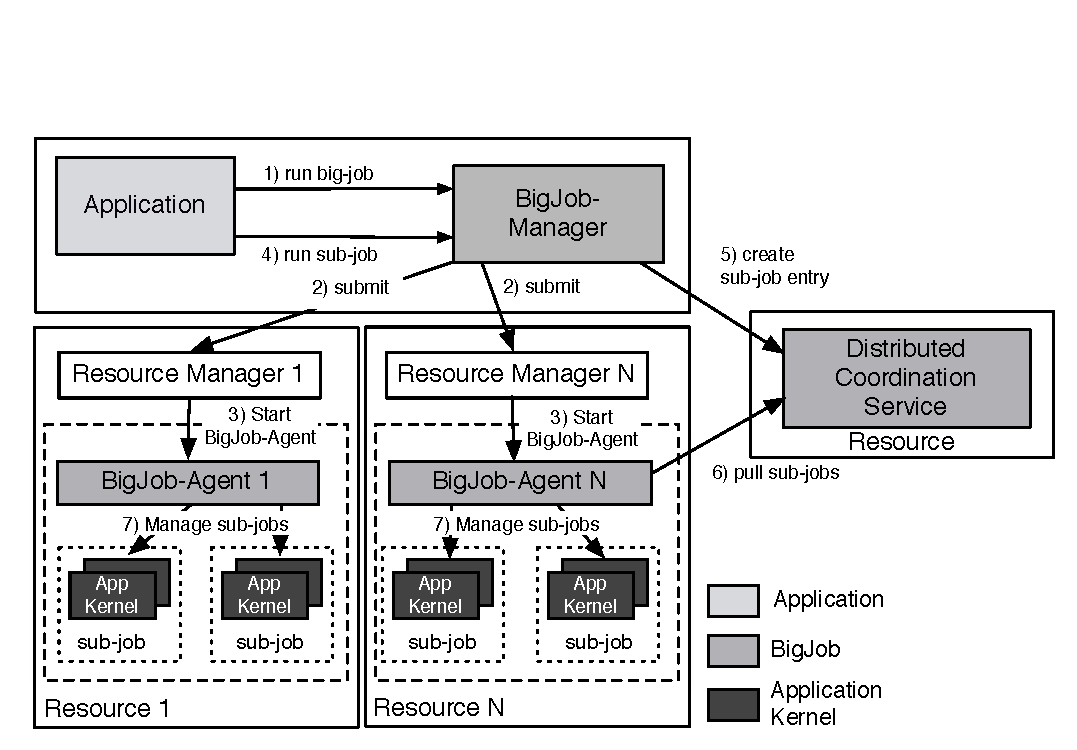
\includegraphics[width=0.45\textwidth]{figures/re_bigjob_interactions.pdf}
	\caption{\I{\textbf{BigJob Architecture and Mapping to P*:}} The
          BJ architecture resembles many elements of the P* Model. The
          BigJob-Manager is the central Pilot-Manager, which
          orchestrates a set of \pilots. Each \pilot is represented by a
          decentral component referred to as the BigJob-Agent. Sub-job
          -- the \cus -- are submitted via the PM. \cus are mapped 1:1
          to \sus.\up\up}
	\label{fig:figures_re_bigjob_interactions}
	%
\end{figure}



\subsection{Condor-G/Glide-in}

The Condor project pioneered the concept of Pilot-Jobs by introducing the
\textit{Condor-G/Glide-in} mechanisms~\cite{condor-g} which allow the
temporary addition of Globus GRAM controlled HPC resources to a Condor
resource pool. The \pilot is exposed as a complete Condor
pool that is started via the Globus GRAM service of a resource. This mechanism
is referred to as Condor Glide-in. Subsequently, jobs (CUs) can be submitted
to the Condor Glide-in pool via standard Condor tools and APIs.

GlideinWMS~\cite{5171374} is a higher-level workload management system built on 
top of the \pilot capabilities of Condor-G/Glide-in. The system can based on 
the current and expected number of jobs in the pool, automatically increase or 
decrease the number of active Glide-ins (\pilots) available to the pool. In 
contrast to Condor-G/Glide-In, the \pilot capabilities are not directly exposed 
to the end-user. GlideinWMS is the recommended mode for accessing OSG resources.


%
%
%
%
%
%
%
%
%
%
%
%
%
%
%
%
%
%
%
%
%
%
%

%
%
%
%


\subsection{DIANE}
DIANE~\cite{Moscicki:908910} is a task coordination framework, which
was originally designed for implementing master/worker applications,
but also provides PJ functionality for job-style executions. it
utilizes a single hierarchy of worker agents and a PJ manager referred
to as \texttt{RunMaster}.  For the spawning of PJs a separate script,
the so-called submitter script, is required. For access to the
physical resources the GANGA framework~\cite{Moscicki20092303} can be
used.  Once the worker agents are started they register themselves at
the RunMaster.  For communication between the RunMaster and worker
agents point-to-point messaging based on
CORBA is used. CORBA is also used for file
staging.  DIANE includes a simple capability matcher and FIFO-based
task scheduler.  Plugins for other workloads, e.\,g.\ DAGs or for
data-intensive application, exist or are under development. 
%
%
%


\subsection{BigJob and BigData: A SAGA-based PJ Framework}
\label{sec:bigjob_description}


%
%
%
%


%
%

%

%
%
%
%
%
%
%



   %
    %
    %
    %


%
%

BigJob (BJ)~\cite{bigjob_web,saga_bigjob_condor_cloud_short} is a SAGA-based PJ
framework. BJ has been designed to be general-purpose and extensible. While BJ
has been originally built for HPC infrastructures, such as XSEDE and
FutureGrid, it is generally also usable in other environments. This
extensibility mainly arises from the usage of SAGA~\cite{saga_url,ogf-gfd-90} 
as a common API for accessing distributed resources. 
%
%
%
%
Figure~\ref{fig:figures_re_bigjob_interactions} illustrates the
BJ architecture and its mapping to P*. The architecture reflects
all P* elements: The BJ-Manager is the Pilot-Manager responsible for
coordinating the different components of the frameworks. The
BigJob-Agent is the actual \pilot that is submitted to a
resource. \cus are referred to as sub-jobs. Internally \cus are mapped
1:1 to \sus.

%
%
%

\begin{figure}[t]
	\up\up\upp
	\centering
	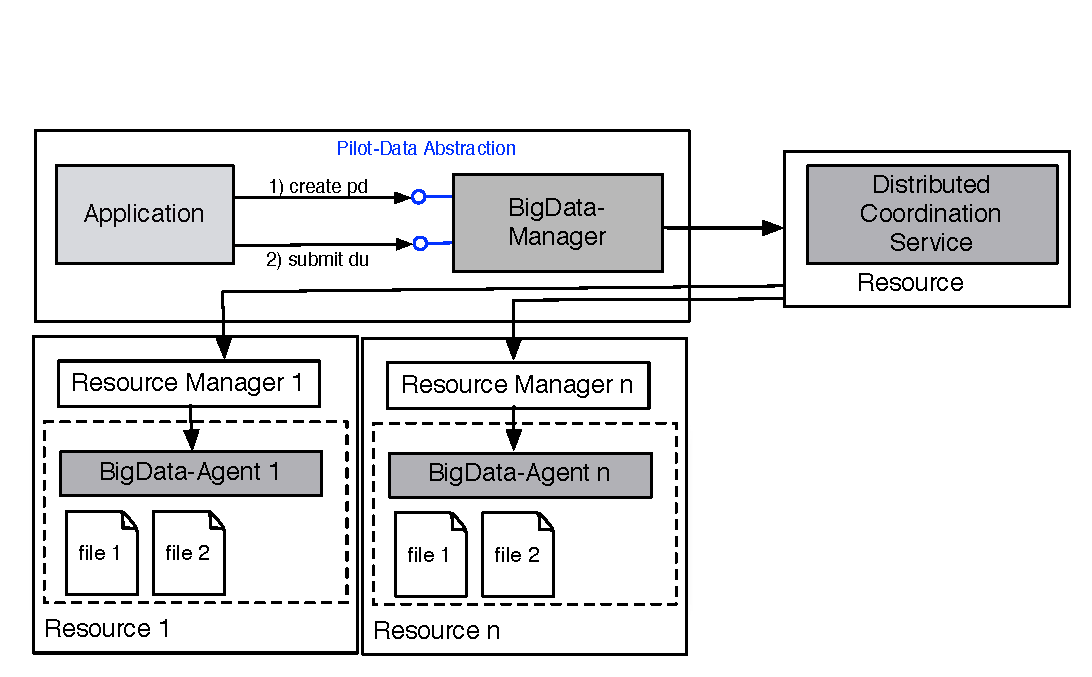
\includegraphics[width=0.42\textwidth]{figures/bigdata_pmr.pdf}
	\caption{\I{\textbf{BigData Architecture and Interactions:}} Similar to BJ, a BD-Manager orchestrates a set of \pilots, i.\,e.\ BigData-Agent. Coordination is carried out via a distributed coordination service. \up\up }
	\label{fig:bigdata}
\end{figure}


BJ implements the following P* characteristic: As coordination model
the M/W scheme is used: The BJ-Manager is the central entity, which
manages the actual \pilot, the BJ-Agent. Each agent is responsible for
gathering local information, for pulling sub-jobs from the manager,
and for executing SUs on its local resource. The SAGA Advert Service
is used for communication between manager and agent. The Advert
Service (AS) exposes a shared data space that can be accessed by
manager and agent, which use the AS to realize a push/pull
communication pattern, i.\,e.\ the manager pushes a \su to the AS while
the agents periodically pull for new SUs. Results and state updates
are similarly pushed back from the agent to the manager. Further, BJ
provides a pluggable communication \& coordination layer and also
supports other \cc systems besides the AS, e.\,g.\ Redis~\cite{redis}
and ZeroMQ~\cite{zmq}.


%

%
%
%
%
%
%
%
%
%
%
%
%
%

{\it BigData (BD)} is an implementation of the Pilot-Data abstraction. BigData
is designed as an extension of BigJob. Figure~\ref{fig:bigdata}
provides an overview of the architecture of BigData. Similar to BigJob, it is
comprised of two components: the BD-Manager and the BD-Agents, which are
deployed on the physical resources. The coordination scheme used is
Master-Worker (MW), with some decentralized intelligence located at the
BD-Agent. The BD-Manager is responsible for (i) meta-data management, i.\,e.\
it keeps track of all \pd and associated \dus, (ii) for scheduling of data
movements and replications (taking into account the application requirements
defined via affinities), and (iii) for managing data movements activities.
BigData supports plug-able storage adaptors (currently for SSH,
WebHDFS~\cite{webhdfs} and Globus Online~\cite{10.1109/MIC.2011.64}).


\begin{table}[t]
\footnotesize
\centering
\begin{tabular}{p{2.4cm}p{1cm}p{1cm}p{1.95cm}p{2.0cm}}
  \toprule
  \textbf{P* Element}    &\textbf{BigJob} &\textbf{DIANE} &\textbf{Condor-G/ Glide-in}     \\\midrule
  Pilot-Manager          &BigJob Manager  & RunMaster     & condor\_master\newline 
                                                            condor\_collector\newline 
                                                            condor\_negotiator\newline 
                                                            condor\_schedd                        \\\midrule
  \pilot                 &BigJob Agent    & Worker Agent  &condor\_master\newline
                                                           condor\_startd                         \\\midrule
  \computeunit  \ (CU)   &Task            &Task           &Job                           \\\midrule
  Scheduling Unit (\su) &Sub-Job         &Task           &Job                           \\\bottomrule
%
%
 \end{tabular}
 \caption{\I{\textbf{Mapping P* elements and PJ Frameworks:} While each PJ framework maintains its own vocabulary, each of the P* elements can be mapped to one (or more) components of the different PJ frameworks.
 }\up\up} 
 \label{table:bigjob-saga-diane}
\end{table}


%
%
%
%
%
%
%
%
%
%
%
%

%


%
%
%
%
%
%
%
%






%
%
%
%
%
%
%
%
%
%
%
%
%
%
%
%
%
%
%
%
%
%
%
%
%
%
%
%
%

%
%
%
%
%
%
%

\subsection{Discussion}

P* provides an abstract model for describing and understanding PJ
frameworks, i.e., different components of PJ frameworks can be mapped
to the P* elements.  While each of the frameworks maintains its own
vocabulary, all share the common P* elements.
Table~\ref{table:bigjob-saga-diane} summarizes how P* can be applied
to BigJob, DIANE and Condor-G/Glide-in.
Table~\ref{table:pilot-job-comparison} summarizes the P*
characteristic and other properties of these frameworks. While most of
these frameworks share many properties, such as the M/W coordination
model, they differ in characteristics, such as communication model
or scheduling. Despite of the many commonalities, the different PJ frameworks 
have different usage modalities mainly cause by the fact that each PJ 
framework  has evolved in a specific infrastructures, e.\,g., 
Condor-G/Glide-in is the native PJ framework of the Open Science Grid.

%
%


%
%
%


%
%
%
%
%
%
%


%
%
%




%
%
%
%
%
%
%
%
%
%
%
%
%
%
%


%
%
%
%

%
%
%


%

%
%
%
%

%
%
%
%

\begin{table}[t]
\footnotesize
\centering
\begin{tabular}{p{1.9cm}p{1.7cm}p{1.6cm}p{1.6cm}}
	\toprule
	\textbf{Properties}
	&\textbf{BigJob} &\textbf{DIANE} &\textbf{Condor-G/\newline Glide-in}    
	\\ \midrule

\textbf{Coordination} &M/W  &M/W &M/W \\ \midrule
	
\textbf{Communication} &Advert Service &CORBA &TCP\\ \midrule

%
%
\textbf{Scheduling} &FIFO, custom &FIFO, custom &Matchmaking, priority-based scheduler \\

%


\midrule
Agent Submission &API &GANGA Submission Script &Condor CLI 
\\

\midrule

End User Environment &API &API and\newline M/W Framework  &CLI Tools \\ 

\midrule

Fault Tolerance &Error propa-\newline gation &Error propa-\newline gation, retries &Error propa-\newline gation, retries \\

\midrule

Resource Abstraction &SAGA &GANGA/\newline SAGA &Globus \\ 

\midrule

Security &Multiple\newline (GSI, User/Pass.) &Multiple (GSI) &Multiple\newline (GSI, 
Kerberos) \\ 

\bottomrule

%
%
%
%

	
\end{tabular}
\caption{\I{\textbf{P* Characteristics and Properties of Different Pilot-Job 
      Frameworks:} The properties
    in bold-face correspond to the P* characteristics; other items are general 
    properties. The PJ frameworks share many P* characteristics and 
    properties, e.\,g.\ the common usage of the M/W scheme or of a 
    resource abstraction layer. However, they also differ in aspects, such as  
    the coordination model or the communication framework. 
    %
    \upp
  }\up\up}
\label{table:pilot-job-comparison}
\end{table}



%
%
%

%

\section{Pilot-API: A Uniform API to Heterogeneous PJ Frameworks}
\label{sec:pilot-api}


%

%
%
%
%
%

In the previous two sections we presented successively the P* Model
and existing Pilot-Job frameworks. Before we present the Pilot-API --
which provides an abstract interface to Pilot-Job frameworks that
adhere to the P* Model, we will motivate the need for such an API.

\subsection{Motivation} 


%
%
%
%
%
%

%
%
%

%
%
%
%
%


%
%
%
%
%
%
%
%
%
%
%
%
%
%
%
%
%
%
%
%
%
%
%
%
%

%

At a high-level, there exist two approaches towards interoperability:
(i) deep integration of systems (system level interoperability), and
(ii) the use abstract interfaces (application level interoperability).
Approach (i) requires a certain level of semantic harmonization
between the systems, and is (in principle and technically) hard to
achieve post-facto, even if the respective systems inherently
implement the same abstract model (here: the P* Model).  While
interoperation via an abstract interface (ii) (here: Pilot-API) is a
semantically weaker approach than (i), it does allow for
interoperability with minimal (application level)
effort~\cite{saga_bigjob_condor_cloud_short,saga_gin}.


%
%
%
%

%
%
%
%
%
%
%
%
%
%
%
%
%
%
%
%
%
%
%
%
%

%
%
%


%
%
%
%
%
%
%
%
%

%
%
%

We appreciate the difficulty of designing an API for multiple, heterogeneous
systems with the right level of semantic expressivity and
simplicity~\cite{Lampson:1983:HCS:800217.806614}. Defining the API as
'smallest common denominator' is often too simplifying and misses large
numbers of 'edge' use cases; defining the API as 'greatest common factor'
clutters the API with non-portable semantics, making the API too
complex~\cite{leaky_abstractions}. The Pilot-API uses the Pareto principle as
guideline for a balanced abstraction level.





%
%
%
%
%
%


%
%
%

%
%
%
%
%
%
%
%

%
%
%
%
%
%
%
%
%
%
%
%

\upp
\subsection{Understanding the Pilot-API}

%
%

The Pilot-API~\cite{pilot_api} is a Python-based API and supports two different 
usage modes (i) it provides a unified API to various PJ frameworks (e.\,g.\ 
BigJob, DIANE and Condor-G/Glide-in), and (ii) it enables the concurrent usage 
of multiple PJ frameworks. The Pilot-API classes and interactions are designed 
to reflect the P* elements and characteristics. 
%
%
The API exposes the two primary interfaces: the 
\texttt{Pilot\-Compute\-Service} is responsible for the management of \pilots 
and the \texttt{Compute\-Unit\-Service} for the management of \cus. As defined 
by P*, a \cu represents a primary self-containing piece of work that is 
submitted through the Pilot-API.



%
%

Figure~\ref{fig:figures_pilot_api_flow} shows the interactions between the
Pilot-API entities. The Pilot-API decouples
workload management and resource scheduling by exposing two separate services: 
The \texttt{Pilot\-Compute\-Service} and
\texttt{Compute\-Unit\-Service}. 
The \texttt{Pilot\-Compute\-Service} serves as a factory for creating \pilots. 
Also, it can be used to query for currently
active \texttt{Pilot\-Compute} instan\-ces.
A \texttt{Pilot\-Compute} instance is returned as result of the
\texttt{create\_pilot()} method of the \texttt{Pi\-lot\-Compute\-Service} (step 1).
The instantiation of the
\texttt{Pilot\-Compute} instance is done by using a
\texttt{Pilot\-ComputeDescription}. The description can be reused and has no
state, while the \texttt{Pilot\-Compute} instance has state and is a reference
for further usage:
the references \texttt{Pilot\-Compute} object represents a \pilot instance and allows the 
application to interact with it, e.\,g.\ to query its state or to cancel 
it. The process of \texttt{Pilot\-Compute} creation is depicted in step 1-2 of 
Figure~\ref{fig:figures_pilot_api_flow} and in Listing~\ref{lst:pcs_creation}.\\


\lstset{
language=Python,
frame=single,
captionpos=b,
stringstyle=\ttfamily,
basicstyle=\scriptsize\ttfamily
}

\begin{minipage}{0.45 \textwidth}
\begin{lstlisting}[caption={\I{Creation of a \T{PilotCompute} instance using a \T{Pi\-lot\-Compute\-Description}.}}, label={lst:pcs_creation}]
pcs = PilotComputeService()
pc_desc = PilotComputeDescription()
pc_desc.total_core_count = 8
pc = pcs.create_pilot('gram://queenbee', 
                          pc_desc, 'bigjob')
\end{lstlisting}
\end{minipage}

Listing~\ref{lst:cus_creation} shows the creation of
a \texttt{Compute\-Unit\-Service}.  Having created
a \texttt{Compute\-Unit\-Service} instance, \texttt{Pilot\-Compute\-Service}
instances can be added and removed at any time, which makes the respective pilots available to that Service.  These semantics enable applications to
respond to dynamic resource requirements at runtime, i.\,e.\ additional
resources can be requested on peak demands, and can be released if they are no
longer required.\\

\begin{minipage}{0.45 \textwidth}
\begin{lstlisting}[caption={\I{Instantiation
of a \texttt{ComputeUnitService} using a reference to the
\texttt{PilotComputeService}.}}, label={lst:cus_creation}]
cus = ComputeUnitService()
cus.add(pcs)
\end{lstlisting}
\end{minipage}

%
%
%

The \texttt{Compute\-Unit\-Service} is responsible for managing the execution of
\cus.
Regardless of the state of the \texttt{Pilot\-Compute\-Service}, applications can submit \cus to a
\texttt{Compute\-Unit\-Service} at anytime (Listing~\ref{lst:submission} and step 3
in Figure~\ref{fig:figures_pilot_api_flow}). 
Once the \texttt{Compute\-Unit\-Service} becomes responsible for a \cu, the \cu
transitions to an \su.
SUs are internally processed (e.\,g.\ they can be aggregated) and are then scheduled to the Pilot-Job Framework (step 4). 
The PJ framework is responsible for the actual execution of the \su on a
resource.
Note that multiple levels of (hierarchical) scheduling can be present -- commonly
a \su is scheduled inside a PJ framework, the model allows it to be present
in multiple layers.\\

\begin{minipage}{0.45 \textwidth}
\begin{lstlisting}[caption={\I{Instantiation and 
	submission of a \texttt{Compute\-Unit\-Description}.}}, label={lst:submission}] 
cud = ComputeUnitDescription()
cud.executable = '/bin/bfast'
cud.arguments = ['match', '-t4', '/data/file1']
cud.total_core_count = 4
cu = cus.submit(cud)
\end{lstlisting}
\end{minipage}



%
%
%
%
%
%
%
%
%
%
%
%
%
%
%
%
%
%
%


Each \texttt{Compute\-Unit} and \texttt{Pilot\-Compute} object is associated
with a state.
The state model is well-defined.
%
Applications can query the state using the \texttt{get\_state()} method or 
they can subscribe to state update notifications using callbacks.

Finally, an application can have any number of \texttt{Pilot\-Compute\-Service} or
\texttt{Compute\-Unit\-Service} instances.
Multiple \texttt{Pilot\-Compute\-Service} instances can be associated to a
\texttt{Compute\-Unit\-Service}, and a \texttt{Pilot\-Compute\-Service} can be associated to
multiple \texttt{Compute\-Unit\-Service} instances.
A \texttt{Compute\-Unit\-Service} can manage multiple \texttt{Compute\-Unit}
instances, but a \texttt{Compute\-Unit} can only be managed by one
\texttt{Compute\-Unit\-Service}.
Similarly, a \texttt{Pilot\-Compute\-Service} can manage multiple
\texttt{Pilot\-Compute} instances, but a \texttt{Pilot\-Compute} can only be
managed by one \texttt{Pilot\-Compute\-Service}.


\begin{figure}[t]
	\centering
  \upp\up\upp
		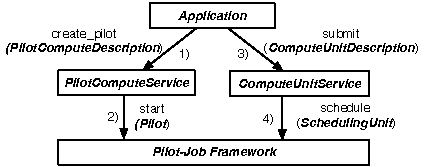
\includegraphics[width=0.4\textwidth]{figures/pilot-api-flow.pdf}
	\caption{\I{\textbf{Control Flow Pilot-API and PJ Frameworks:} The 
	functionality of pilot-jobs are exposed using two primary classes: The 
	\texttt{Pilot\-Compute\-Service} for the management 
	of \pilots, and the \texttt{Compute\-Unit\-Service} for the management of 
	\cus. \up
	}}
	\label{fig:figures_pilot_api_flow}
\end{figure}

%
%
%
%
%
%
%
%
%
%
%
%
%
%
%
%
%


\subsection{Pilot-API for Data}

Analogous to the Pilot-API for Compute, the Pilot Data
API~\cite{pilot_api} defines the \texttt{PilotDataService} entity as
an abstraction for creating and managing pools of storage. A
\texttt{PilotData} instance represents the actual physical storage
space. An additional \texttt{ComputeDataService} entity functions as an
application-level scheduler, which accepts both
\texttt{Compute\-Units} and \texttt{DataUnits} -- this resolves new
dependencies (e.g. data/data or data/computer affinities), and is
responsible for managing the execution of \dus and \cus.\\
\\
In summary, the Pilot-API provides a well-defined abstraction for managing
both compute and data. The API has been developed to support production-scale
science on production infrastructure. As shown in
Figure~\ref{fig:figures_distributed_pilot_job} the API supports different HPC
and HTC infrastructures.

%

\begin{figure}[t]

    \begin{center}
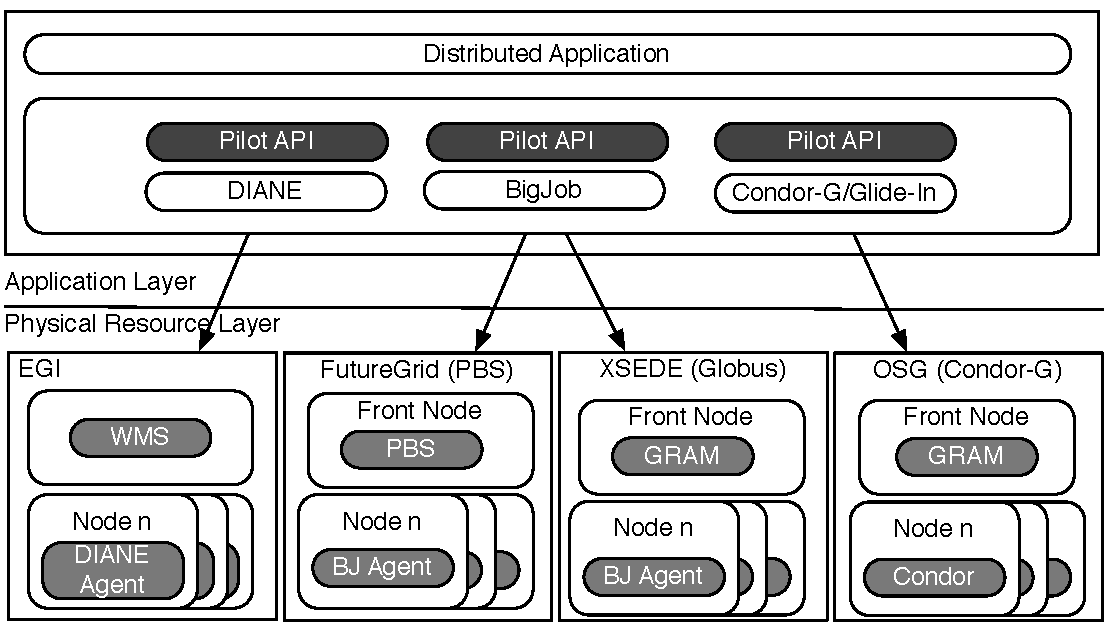
\includegraphics[width=0.38\textwidth]{figures/distributed_pilot_job.pdf}
    \caption{\I{\textbf{Pilot-API and PJ frameworks:} The Pilot-API
        provides a unified interface to utilize the native Pilot-Job
        capabilities of different infrastructures, e.\,g.\ BigJob for
        XSEDE/FutureGrid, DIANE for EGI and Condor for OSG.
  	}\label{fig:figures_distributed_pilot_job}}
	\upp\upp\upp
  \end{center}    
\end{figure}


%
%

%
%
%
%
%
%
%
%
%
%
%
%
%
%


\section{Experiments and Results}\label{sec:exp_res}

%
%
%
%
%
%
%
%
%
%
%
%
%
%
%
%
%
%
%
%
%
%
%
%
%
%
%
%
%
%
%

%
%

As discussed in \S\ref{sec:pilot-job-frameworks}, several PJ
frameworks can be collectively used via the Pilot-API. We begin by
understanding the overhead of PJ frameworks
(section~\ref{sec:pj_performance}). In
section~\ref{sec:fg-xsede-osg-egi} we show the effectiveness of the
Pilot-API/P* Model approach by executing {\it real application
  workloads} -- a genome alignment application -- on multiple distinct
production (XSEDE, EGI, OSG) and research (FutureGrid)
infrastructures. It is important to note that our experiments do not
try to identify the ``fastest'' PJ framework, as this is dependent on
several external factors, often specific to the infrastructure
used. In stead, we focus on demonstrating interoperability via the
common Pilot-API by using multiple PJ frameworks concurrently on
multiple infrastructures (see section~\ref{sec:experiment-interop}).
%
%
Further, we show how \pilotdata enables applications (i) to lower
the volume of the transferred data, and (ii) to utilize different
transfer protocols in section~\ref{sec:experiment-pilotdata}.

%
%
%

%
%
%
%
%
%


%
%
%

%
%
%
%
%
%
%

%
%

%
%



%
%
%
%
%
%
%
%
%


%
%
%
%
%

%
%
%
%

\subsection{PJ Frameworks Overhead}\label{sec:pj_performance}

%
Before we understand the performance of different frameworks for real
application workloads, we analyze the typical overheads for BigJob and
DIANE.  The overhead of a PJ framework, like many distributed
submission mechanisms and tools, is most commonly determined by the
following factors: the API overhead, the job submission and
coordination overhead. Although important determinants of the
time-to-solution, the queueing and file staging time heavily depend on
extrinsic factors, such as the system and network load, but are not
intrinsic overheads of the PJ framework. The overhead of the
API-layer, i.\,e.\ the Pilot-API, was not measurable using the
built-in Python profiler, which provides accuracies in the magnitude
of milliseconds; this places an effective upper-bound on Pilot-API
latencies. Ref.~\cite{saga_europar10-short} established that even in a
distributed context, job submission overheads, are very low when
compared to the runtimes in consideration.  There are many factors
that influence the overall performance, e.\,g.\ the
degree of distribution (local (LAN) vs. remote (WAN)), the
communication pattern (1:n versus n:n) and the communication
frequency. We focus our investigation on the the communication \& 
coordination (\cc) subsystem, which we established earlier as
import characteristics of PJ frameworks.

%
%
%

We executed a different number of very short running (i.\,e. zero
workload) \cus on Alamo/FG concurrently.  This enables us to focus on
the overhead induced by the \cc subsystem. In general, the c\&c
systems used are mostly insensitive to the number of coordinated \cus.
Although we do not provide a detailed discussion of the dependency
between coordination overhead and the number of \cus, it is worth
mentioning that the runtime increases only slightly with the size of
the pilot and/or the number of managed \cus.

%

%
%
%
Figure~\ref{fig:perf_bigjob-varying-cores}
illustrates the scalability of BJ and DIANE with respect to the number
of cores and \cus managed by \pilot. For this purpose, we execute
4\,\cus per core, i.\,e.\ between 32 and 512\,\cus.  BigJob with Redis
(local) shows almost linear scaling up to 128 cores. BigJob with Redis
(remote) imposes an increase of about 14\,\%. BigJob with ZeroMQ
performs very well with lower core counts; with larger core counts,
the runtimes increase, indicating a potential scalability
bottleneck. Due to higher startup overhead, at lower core counts DIANE
shows a longer runtime than ZeroMQ or Redis.  At higher core counts
DIANE behaves similar to BigJob/ZeroMQ, but shows a greater increase
in the overall runtime. This increase is likely attributable to the
single central manager in DIANE's CORBA-based client-server
architecture. Using Redis as central data space for BigJob decouples
Pilot-Manager and Agent, yielding better performance in particular
with many CUs. 

\begin{figure}[t] \centering \up\up
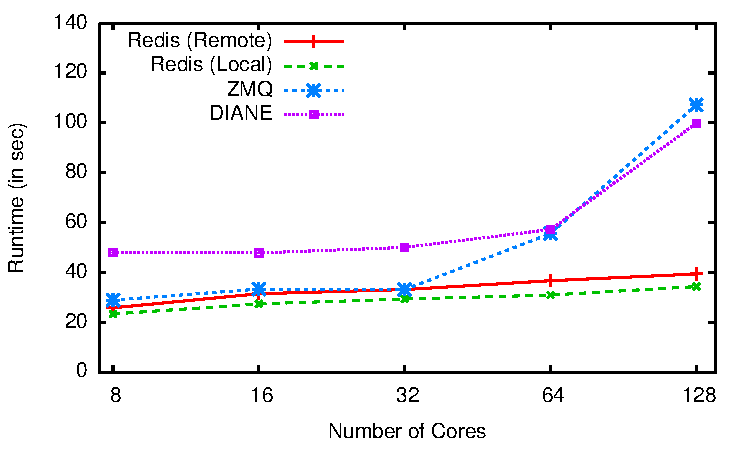
\includegraphics[width=0.4\textwidth]{perf/bigjob-varying-cores-alamo-noadvert-scaled.pdf}
\upp \caption{\I{\textbf{\pilotjob Coordination Mechanism:}  The runtime of a
workload of 4 \cus per core, i.\,e.\ 32 - 512\,\cus, using different \pilots
and configuration. For BJ-Redis the runtime  increases only moderately, the
client-server-based implementations BJ-ZMQ and CORBA-based DIANE show
particularly a steep increase when going from 64 to 128 cores. \up\up }}
\label{fig:perf_bigjob-varying-cores} \end{figure}

%
%
%
%
%
%
%
%
%
%
%
%
%
%
%
%
%
%
%
%
%

\subsection{Characterizing PJ Frameworks on DCI}
\label{sec:fg-xsede-osg-egi}


%

To validate the effectiveness and usability of the Pilot-API, we
conducted a series of experiments on various production
infrastructures. We executed BFAST~\cite{bfast2009} using three
different PJ frameworks (BigJob, DIANE and Condor) on
XSEDE~\cite{xsede}, FutureGrid~\cite{fg}, EGI~\cite{egi} and
OSG~\cite{1742-6596-78-1-012057}.  Specifically, we utilized the
following resources: XSEDE: Trestles (100\,TFlop / 324\,nodes /
10,368\,cores / Torque) and QueenBee (Linux Cluster / 668\,nodes /
5,344\,cores / PBS); FutureGrid: India and Sierra (108\,nodes /
864\,cores / PBS);
EGI: Resource federation of 364,500 cores;
OSG: Condor pool (via the \textit{Engage} VO, GlideinWMS, 20,000
Glide-ins).

%
%
%
%

%
%
%
 
%
%
%
%
%


%
%
%
%
%
%
%
%
%
%
%
%
%
%
%
%
%
%
%
%
%
%
%
%


%
%
%

\subsubsection*{Experimental Configuration}

%
%
%

%
%
%
%
%
%
%
%

We run experiments using five different configurations: (B1) BigJob/XSEDE,
(B2) BigJob/FutureGrid, (B3) two BigJob/Futuregrid, (B4) DIANE/EGI, (B5)
Condor/OSG. As discussed, the Pilot-API provides a unified interface for
accessing these infrastructures using the respective native PJ framework,
i.\,e.\ BigJob, DIANE and Condor (see
figure~\ref{fig:figures_distributed_pilot_job}). For BJ we use the PBS/SSH
plugin to access both the FutureGrid and XSEDE machines. On OSG, we use SAGA
and the SAGA-Condor adaptor to interface directly with OSG's dynamic
GlideinWMS resource pool. Further, we utilize DIANE on EGI.
%
%
%

The investigated workload consists of 128 \cus. Each \cu executes a BFAST
matching process, which is used to find potential DNA sequence alignments.
Each \cu requires the following input data: 1.9\,GB for the
reference genome and index files, and 170\,MB for the \textit{short read}
file (generated by the DNA sequencing machine). A total
of 128 read files (one per CU) are used. Each BFAST \cu requires 1 core; All
input files are staged previous to the actual run.

%
%
%

%
%

%
%

%
%
%
%

%
%
%

%
%
%
%
%
%
%

\begin{figure}[t]
 \up\up
 \centering
 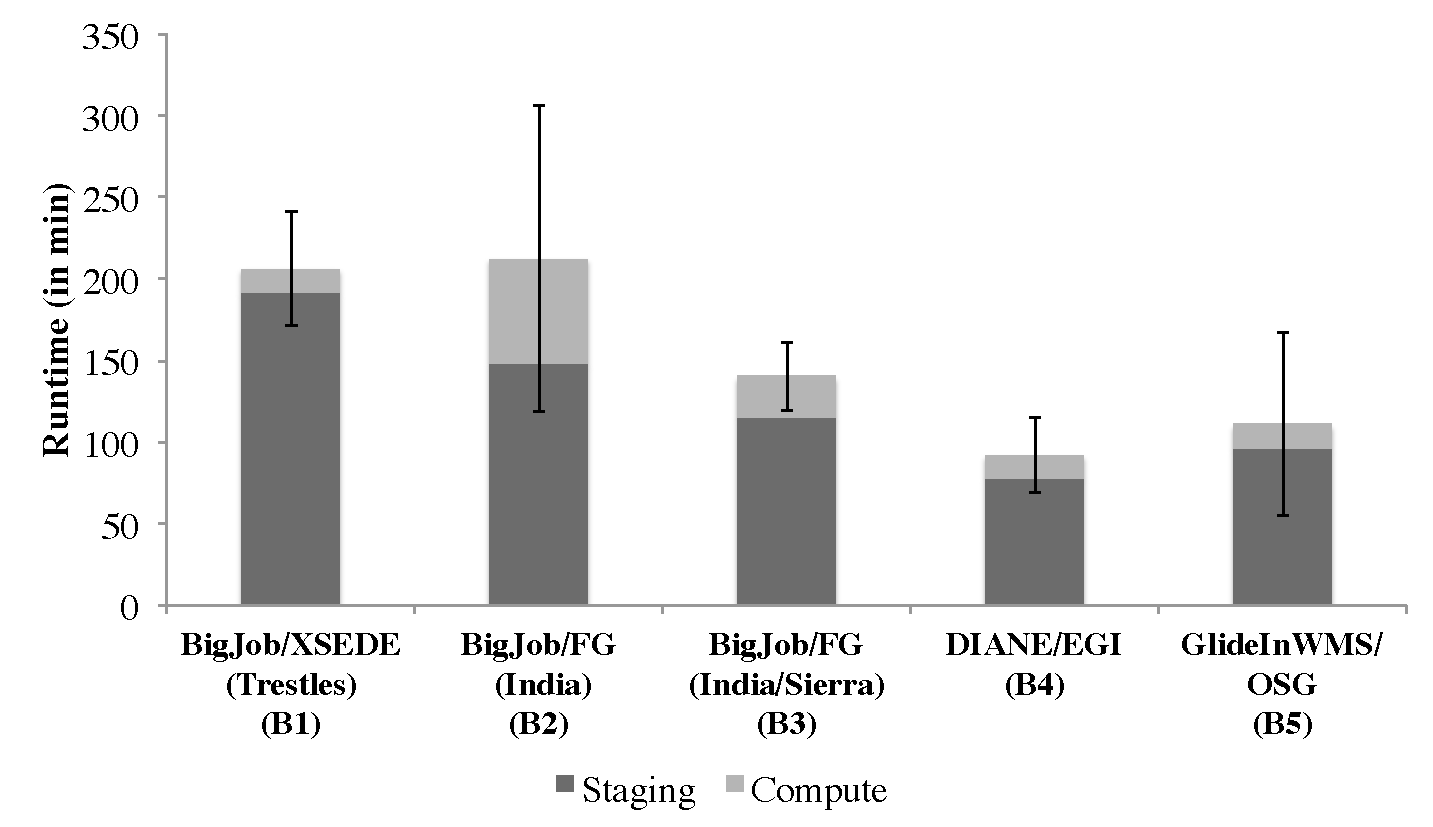
\includegraphics[width=0.42\textwidth]{perf/128-bfast-egi-fg-xsede-osg-with-staging.pdf}
 \caption{\I{\textbf{PJ Framework Performance on XSEDE, FutureGrid, EGI and 
  OSG:} Average runtime of 128 BFAST match tasks on 128 cores. Each experiment
  is repeated at least 3 times.}\up}
%
%
\label{fig:perf_perf-bfast-bj}
\end{figure}

%

\subsubsection*{Experimental Results}

%
%
%

Figure~\ref{fig:perf_perf-bfast-bj} shows the results of the
experiments. We measured the time to transfer input files ($T_X$), and
the compute time $T_C$. $T_C$ also includes the overhead of the pilot.
The total runtime ($T_R$) is the sum of $T_X$ and $T_C$.  For each
\cu, the reference genome, the index files and one read file need to
be staged (1.9\,GB); this constitutes the most significant part of the
overall runtime. In particular, on HPC clusters, the staging quickly
becomes a bottleneck due to the fact that all \cus share the incoming
network bandwidth.  Also, fluctuation of the bandwidth in this
scenario leads to a high failure rate during downloads. As seen in B3
(middle bar), the distribution of the network load to two resources
leads to a reduction of $T_{X}$. Also, in the HTC configuration (B4,
B5), \cus are distributed across multiple machines minimizing the
possibility of network congestions of single links. As an indication,
a typical run of 128 CUs on OSG ended up being scheduled on 10+ sites
spread over an equal amount of nodes per site.

%
%
%
%
%

%

In general $T_{C}$, %
is heavily dependent on the available disk I/O. Both Trestles (XSEDE)
and India/Sierra (FG) have shared network filesystems (Lustre for
Trestles, NFS for India), which are utilized by all jobs running on
these machines. The collective performance of multiple, concurrent
BFAST \cu thus degrades significantly as contention for available disk
I/O bandwidth increases due to larger number of tasks accessing the
filesystem concurrently (due to the usage of NFS, the runtime on India
is depending on the scenario $>$20\,\% slower than other machines). On
EGI and OSG, BFAST \cu performs best. This can mainly be attributed to
the use of local storage and the high degree of distribution of the
\cus to multiple sites.


%
%
%
%
%

%
%
%
%
%
%
%
%
%
%
%
%
%
%


%
%
%
%


%
%
%
%
%




%
%
%
%
%
%
%
%
%


%
%
%
%
%
%

%
%
%


%
%
%
%
%



\subsection{PJ Framework Interoperability}
\label{sec:experiment-interop}

%
%

In principal, two types of interoperability between \pilotjobs and
infrastructure exist: the first is the usage of a given PJ framework
on different infrastructures; in the scenario examined, BigJob is used
on different infrastructures by invoking different SAGA adaptors.  The
second is the usage of distinct PJ frameworks via the Pilot-API, i.e.,
interoperability between PJ frameworks. In configuration C1 we utilize
SAGA adaptors to run BigJob concurrently on FutureGrid:India and
XSEDE:Trestles. C2 and C3 show PJ framework interoperability by
concurrently running BigJob and DIANE on FutureGrid:India and EGI
(C2), as well as Condor and BigJob on OSG and XSEDE:QueenBee (C3). It
is worth reiterating, that to the best of our knowledge, the latter
scenario, wherein different PJ frameworks are utilized concurrently
for the same application (whether on the same infrastructure or
distinct) has never before been realized. We attribute this to the use
of the Pilot-API.  For all scenarios, we run the same BFAST
application described in \S\ref{sec:fg-xsede-osg-egi} with 64\,\cus on
each infrastructure, i.\,e.\ in total 128\,\cus.

\begin{figure}[t]
 \up\up
  	\centering
	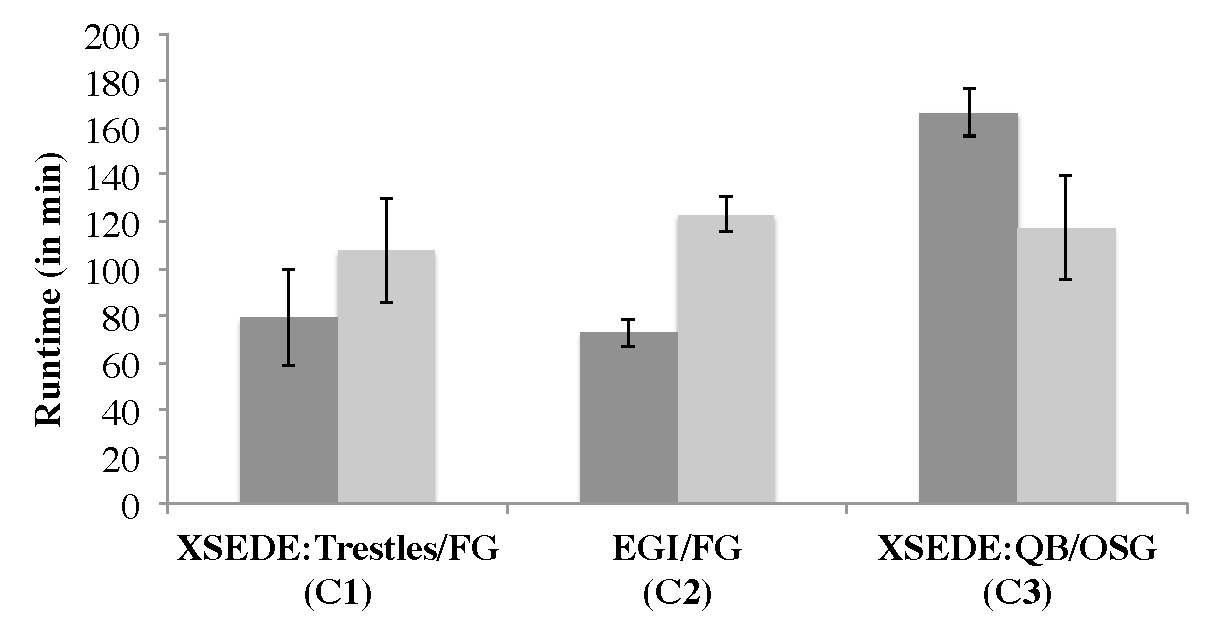
\includegraphics[width=0.42\textwidth]{perf/128-bfast-interop-with-staging.pdf}
	\caption{\I{\textbf{PJ Framework Interoperability:} Average runtime of
          128 BFAST \cus on different infrastructures. \cus are
          equally distributed across the two infrastructures. The
          performance heavily depends on the available bandwidths to
          the resources, which determines the time required for file
          transfers.\up}}
	\label{fig:perf_interop_128-bfast-interop}
\end{figure}


%
%
%

Figure~\ref{fig:perf_interop_128-bfast-interop} shows the results of
the interoperability tests. In C1, one BJ \pilot is submitted to
Trestles and one BJ \pilot to FG/India.  The overall runtime is the
sum of the file staging and the actual compute time on the respective
resource. Consistent with previous results, the \pilot on Trestles
finished before the \pilot on India. $T_R$ of the distributed run
improved more than 50\,\% compared to a run on only one resource,
i.e., Trestles or India only, mainly due to the minimization of the
incoming bandwidth bottleneck by distributing the load to two sites.


%
%

%
%

The middle bar (C2) in Figure~\ref{fig:perf_interop_128-bfast-interop}
demonstrates that two PJ frameworks can be utilized concurrently using
the Pilot-API. As previously, the overall performance heavily depends
on the time required for staging the files (for configuration C2 and
C3 we estimated the staging times based on previous
measurements). Further, some performance overhead is induced by the
distributed coordination necessary particular in case C2 where the BJ
manager and Redis service are highly distributed. In this
configuration, the communication is conducted via a Redis instance
deployed on FG, while the BJ manager is deployed on EGI; thus, for
each \cu several cross-atlantic roundtrips (latencies $>$100\,msec)
are necessary. Another important aspect is file staging: as previously
established, the incoming network bandwidth quickly becomes a
bottleneck as in the FG case (even dominating the distributed
latencies). In HTC environments the pilots and 
\cus, are distributed across multiple machines, which avoids such
bottlenecks.  Finally, C3 (right bars in
Figure~\ref{fig:perf_interop_128-bfast-interop}) shows the result of
the OSG and XSEDE:QB run. Since QueenBee is an older XSEDE machine,
$T_R$ on this machine is much longer than $T_R$ on OSG.

%
%

Although the aim of our experiments is to demonstrate interoperable
use of hitherto distinct and disjoint \pilotjobs, in the process we
highlight the performance advantages that can emanate from the ability
to seamlessly distribute (I/O intensive) workloads in a scalable
manner. The Pilot-API does not represent a barrier to
scalability, but by virtue of facilitating the use of distributed
resources, it provides the ability to overcome limitations to
scalability on certain infrastructure arising from factors such as
I/O, memory, and/or bandwidths. 
%
%
%

\upp
\subsection{Pilot-Data: Data Transfer and Management}
\label{sec:experiment-pilotdata}
%
An important challenge
when running distributed data-intensive tasks is the effective
management of data, and its efficient transfer. We investigate
different scenarios: (D1) the usage of application-level file staging
without PD, (D2) the usage of PD with the SSH plugin, %
%
%
%
and (D3) the usage of PD with Globus
Online. For these experiments, we utilize Trestles (XSEDE). The input
files are located on a remote machine: Quarry (IU) for D1; Lonestar
(TACC) for D2 and D3.


\begin{figure}[t]
	\upp
	\centering
		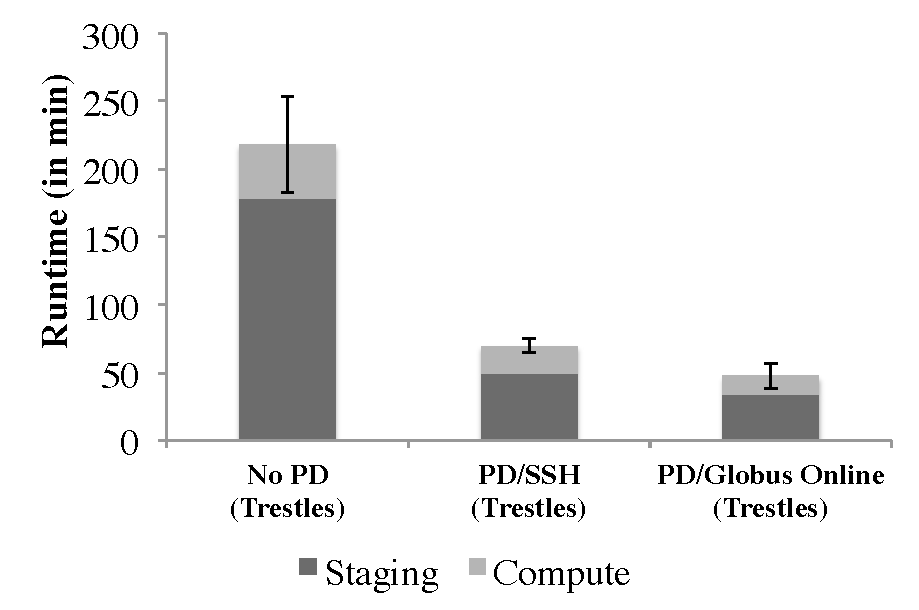
\includegraphics[width=0.4\textwidth]{perf/pd-128cus.pdf}
	\caption{\I{\textbf{Pilot-Data (PD) Performance:} Using PD the staging 
	time can be significantly improved due to a reduction of the overall data 
	transfer volume from 128 times 1.9\,GB to about 24\,GB (1.9\,GB + 128 
	times 170\,MB). Further, Globus Online utilizes with GridFTP a more 
	efficient transfer protocol.\up\up}}
	\label{fig:perf_sc_download-concurrent-cus}
\end{figure}

%

As previously alluded
(Figure~\ref{fig:perf_interop_128-bfast-interop}), as the number of
CUs increases, file staging quickly becomes a bottleneck, as all CUs
share the incoming bandwidth.  Also, I/O contention on the shared file
systems leads to an increasing compute time.
Figure~\ref{fig:perf_sc_download-concurrent-cus} shows that with an
increasing number of CUs, the naive way of moving files (D1) is not a
scalable solution; this is reflected in a runtime of $>$4 hours for 128
CUs.  While the download time increases linearly with the number of
CUs, the compute time remains almost constant at $\sim$15\,min.

There are two options to address this issue: (i) distribute/scale-out
the computation to multiple resources (C3), and/or (ii) optimize data
transfers using PD.  The optimization via PD 
has two components: the amount transferred and the transfer protocol.  By
being cognizant of the distribution of the \cus, redundant transfers
can be reduced (if not eliminated); using PD the overall
amount of data that needs to be transferred for the 128 CU scenario
can be reduced from 243\,GB (i.\,e.\ 128\,\cus times 1.9\,GB data for
the reference genome, index files and 1 read file) to 24\,GB (a single
transfer of the reference genome and index files and 1 read file per
\cu, i.\,e.\ 128 times 170\,MB).  The staging times in D2 and D3 are
significantly lower than in D1. Further, Globus Online show a
significant better performance than SSH ($\sim$30\,\%) mainly due to
the usage of a more efficient transfer protocol (GridFTP).

%
%
%
%

%
%

%
%
%

%
%
%
%
%
%
%

%
%

%
%
%

\section{Discussion and Future Work}

\label{sec:discussion-future-work}
%
%
%
%
%
%

%

The primary intellectual contributions of this work are (i) the
development of the P* Model, (ii) the mapping of the P* elements to PJ
frameworks such as Condor-G/Glide-in, and (iii) the design and
development of the Pilot-API.  The P* Model provides a common abstract
model for describing and characterizing Pilot-abstractions; the
Pilot-API exposes the P* elements and characteristics.  We validate
the P* Model by demonstrating that the most widely used PJ frameworks,
viz., DIANE and Condor-G/Glide-in, can be compared, contrasted and
analyzed using this analytical framework.  Furthermore we demonstrate
the use of the Pilot-API with multiple PJ frameworks on distributed
production cyberinfrastructure, such as XSEDE, OSG, EGI and
FutureGrid.

Although current PJ frameworks collectively support millions of tasks
yearly on several production distributed infrastructure, extensibility
and interoperability remain a significant challenge~\cite{extenci}. In
addition, there is confusion about what constitutes a \pilotjob
system; in the absence of a well-defined model, often different
semantic capabilities and functionality are compared. For example, 
GlideinWMS is often called a \pilotjob, which is then logically
compared to DIANE or BigJob. Using the P* Model, one can address this
ambiguity and clearly establish that GlideinWMS provides a specific
{\it scheduling} characteristic for an implementation of the
Condor/Glide-in \pilotjob. 
%
%
%
%
%

This points to the first non-trivial deduction that this paper makes:
it presents, arguably for the first time, an analytical framework upon
which to construct {\it tools} and thereby define them as
implementations of a specific and semantically well-defined
capability, rather than a loosely-defined capability validated by a
weak existence principle, i.\,e., ``because it exists, it must be
correct''. One can argue that similar semantic tightness is required
in the implementation and definition of middleware capabilities.  The
second non-trivial deduction is that this paper presents a conceptual
framework which unifies job and data abstractions, via an extended and
generalized \pilot abstraction.  Given the increasing importance of
\pilotjobs in supporting scalable dynamical execution and the
challenges associated with distributed data placement, this
%
%
has immense practical implications and potential. 
%
%
%

However, the other practical implications of this work are already
evident: the Pilot-API~\cite{pilot_api} has been deployed to support
production-scale science on production infrastructure as emphasized 
in our experimentation. In fact, it is a stated goal of our research to
enhance the range of applications and usage-modes that will benefit
from the \pilot abstraction, by deeply integrating Pilot-API/P*
capabilities with multiple production infrastructures (both grids and
clouds).  However, attention to several deployment issues is required,
e.\,g., in spite
of a common Pilot-API, each PJ framework has a rather different usage
modality; this is reflective of the fact that typically, PJ frameworks
``evolve in'' and are ``native to'' specific infrastructure, e.g.,
Condor-G/Glide-in is the native PJ framework of the OSG, and its use
is heavily coupled with infrastructure specific to OSG, such as
GlideinWMS. This is not a limitation of our approach, but a
reiteration of the need for the P* approach as a first-step in
addressing deployment barriers towards interoperability.

%
%
%
The \pilotjobs concept is not limited to traditional distributed CI but also
has applicability to Clouds. For example, PaaS cloud systems, such as Venus-C
(Azure), support the notion of Generic Workers (worker role) which are
conceptually similar to pilots in that they pull tasks (application workload)
from a {\it central repository} when the environment is available.
Furthermore, \pilotjobs map well to Iaas cloud systems, wherein a \pilot can
marshall multiple VMs, possibly of different characteristics and performance
capabilities; an agent which pulls and executes \cus is deployed on each VM.
Ultimately, there is a decoupling between task specification and resource
assignment, with the \pilot-Manager or an equivalent cloud-entity carrying 
out the mapping using dynamic/real-time information.
The specifics of matching \cus to clouds is distinct from the
matching \cus to grids.

P* provides significant future development \& research opportunities, e.\,g.,
to experiment and reason on the relative roles of system versus
application-level scheduling, heuristics for dynamic execution, the role of
affinity and data/compute placement strategies, to name just a few. We will
explore these ideas in upcoming work and integrate the results with
production-grade implementations.


%
%

%
%
%
%

%
%

%
%
%
%
%

%


%
%

%
%

%
%
%
%
%
%
%

%
%
%

%
%

%
%


%
%
%
%

%
%
%
%

%
%
%
%
%
%
%
%
%
%
%
%
%
%
%

%
%
%

%
%
%
%
%


%
%
%
%
%


%
%
%
%
%
%
%
%
%


%
%
%

%
%
%

%
%

%
%
%

%
%
%
%
%
%
%
%
%

%
\section*{Acknowledgements}
%
\footnotesize \footnotesize{This work is funded by NSF CHE-1125332
  (Cyber-enabled Discovery and Innovation), HPCOPS NSF-OCI 0710874
  award, NSF-ExTENCI (OCI-1007115) and NIH Grant Number P20RR016456
  from the NIH National Center For Research Resources. Important
  funding for SAGA has been provided by the UK EPSRC grant number
  GR/D0766171/1 (via OMII-UK) and the Cybertools project (PI Jha)
  NSF/LEQSF (2007-10)-CyberRII-01, NSF EPSCoR Cooperative Agreement
  No. EPS-1003897 with additional support from the Louisiana Board of
  Regents.  SJ acknowledges the e-Science Institute, Edinburgh for
  supporting the research theme. ``Distributed Programming
  Abstractions'' \& 3DPAS. MS is sponsored by the program of BiG Grid,
  the Dutch e-Science Grid, which is financially supported by the
  Netherlands Organisation for Scientific Research, NWO. SJ
  acknowledges useful related discussions with Jon Weissman
  (Minnesota) and Dan Katz (Chicago). We thank J Kim (CCT) for
  assistance with BFAST.  This work has also been made possible thanks
  to computer resources provided by TeraGrid TRAC award TG-MCB090174
  (Jha) and BiG Grid.  This document was developed with support from
  the US NSF under Grant No. 0910812 to Indiana University for
  ``FutureGrid: An Experimental, High-Performance Grid Test-bed''.}

  
%
%
\bibliographystyle{IEEEtran}
\bibliography{../pilotjob,../saga,../saga-related}


\end{document}

%
%

%
%

%
%
%
%

%
%
%
%
%
%

%
%
%
%
%

%
%
%
%
%
%
%
%
%
%
%

%
%
%

%
%
%
%
%
%
%
%
%
%
%

%
%
%
%
%
%
%
%
%
%
%

%
%

%
%
%
%

%
%
%
%

%
%
%


%
%
%
%
%
%
%
%
%
%
%
%
%
%
%
%
%
%
%
%
%
%
%
%
%
%
%
%
%
%
%
%
%
%
%

%
%
%
%
%
%
%
%
%
%

%
%
%


%
%
%
%
%
%
%
%

%
%
